%! Author = BartoszW
%! Date = 3/9/2020

\documentclass[a4paper,12pt]{article}

% Packages
\usepackage{amsmath}
\usepackage[T1]{fontenc}
\usepackage[polish]{babel}
\usepackage[utf8]{inputenc}
\selectlanguage{polish}
\usepackage{lmodern}
\usepackage{amsfonts}
\usepackage{hyperref}
\usepackage{graphicx}
\usepackage{float}
\usepackage[margin=1in]{geometry}

% Document
\begin{document}

    \title{Sprawozdanie Lab1 - UAI}
    \author{Bartosz Walusiak, Krzysztof Zdulski}
    \date{\today}
    \maketitle

    \tableofcontents
    \newpage

    \section{Cel Ćwiczenia}\label{sec:cel-ćwiczenia}

    Celem ćwiczenia laboratoryjnego było użycie narzędzia PragmaDev oraz języka SDL do zbudowania prostego systemu
    odpowiadającego na żądania użytkownika.


    \section{Przebieg zadania}\label{sec:przebieg-zadania}

    \subsection{Podstawy Obsługi Narzędzia PragmaDev}\label{subsec:podstawy-obsługi-narzędzia-pragnadev}

    Na początku laboratorium nauczyliśmy się obsługiwać GUI PragmaDev, poznaliśmy elementy takie jak: tworzenie nowego
    projektu, dodawanie/usuwanie/modyfikowanie elementów systemu, obsługa poszczególnych okienek odpowiadających za
    funkcjonowanie i symulację działania systemu.

    \subsection{Budowa Systemu}\label{subsec:budowa-systemu}

    \begin{figure}[H]
        \centering
        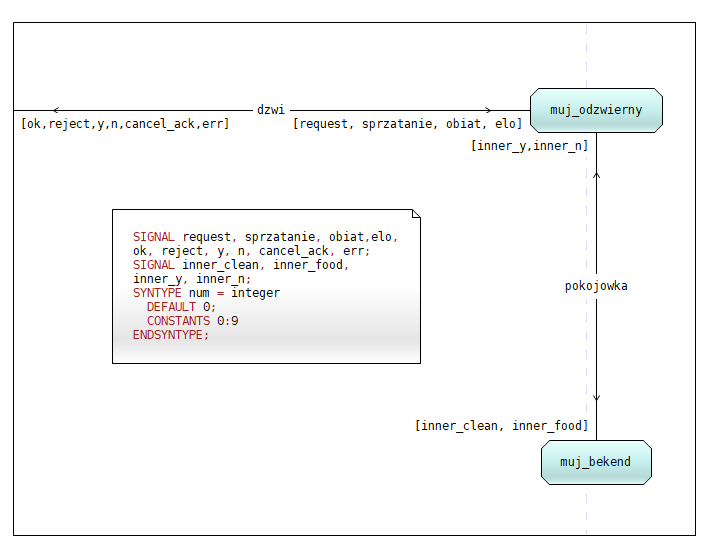
\includegraphics[width=1\textwidth]{images/system.png}
        \caption{muj\_system}
    \end{figure}

    \newpage

    Wykorzystując nowo poznane narzędzie zaprojektowaliśmy system który:
    \begin{itemize}
        \item Oczekuje na żądanie użytkownika
        \item Odpowiada \texttt{ok} albo \texttt{reject} losowo z szansą $\frac{1}{10}$ na niepowodzenie, symulując tym samym nieprzewidziane problemy.
        \item W zależności od dalszego działania użytkownika wykonuje żądanie lub odmawia usługi z uwagi na niedostępne zasoby, na potrzeby symulacji określane losowo.
        \item Posiada możliwość przerwania usługi w dowolnym momencie jej wykonywania.
        \item odpowiada błędem na nowe żądania gdy system jest zajęty - symulacja zajętości za pomocą timer'a.
    \end{itemize}

    \begin{figure}[H]
        \centering
        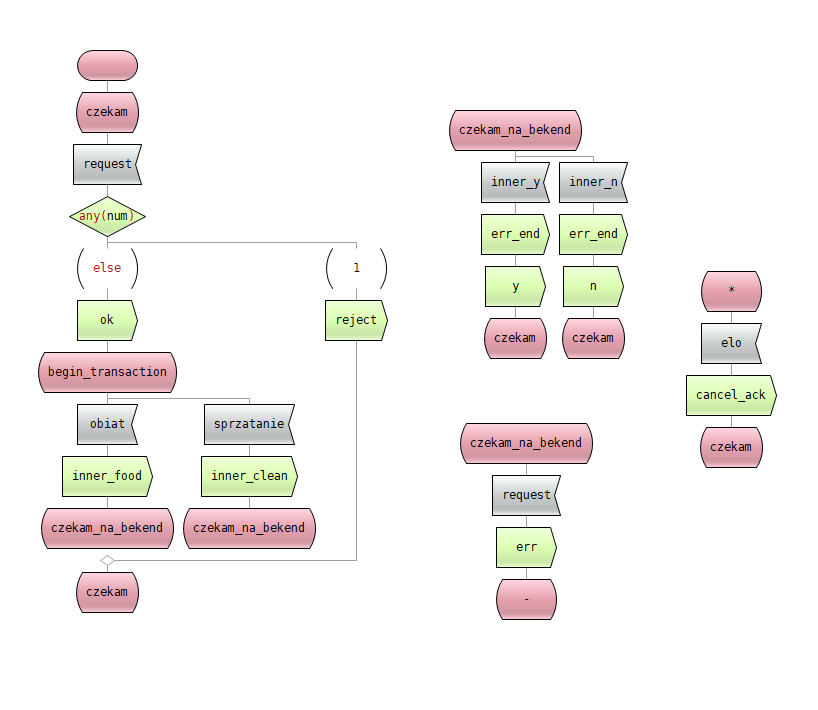
\includegraphics[width=0.6\textwidth]{images/process1.png}
        \caption{muj\_odzwierny}
    \end{figure}

    \begin{figure}[H]
        \centering
        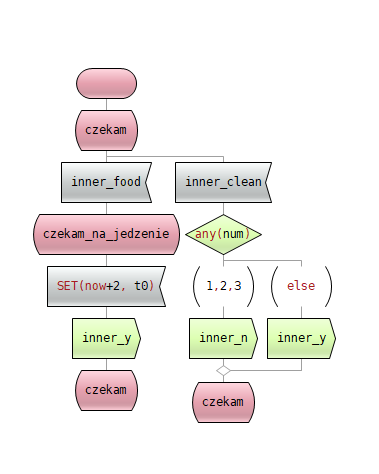
\includegraphics[width=0.3\textwidth]{images/process2.png}
        \caption{muj\_bekend}
    \end{figure}


    Dbając o komfort wizualny użytkownika nadaliśmy projektowi stylistykę drzwi.

    \begin{figure}[H]
        \centering
        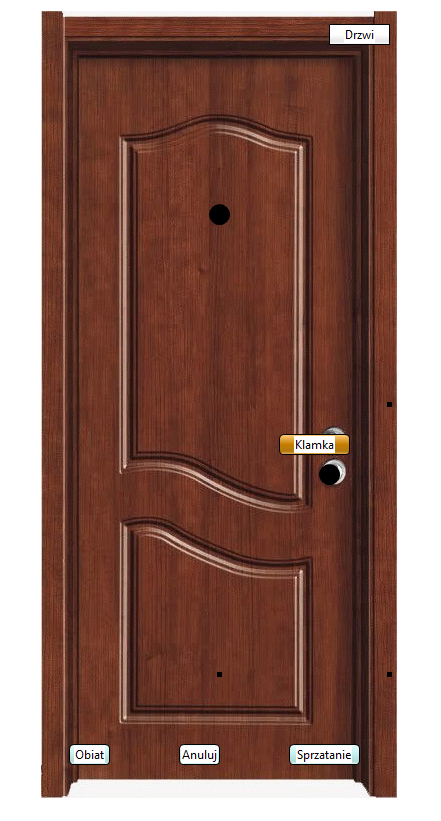
\includegraphics[width=0.4\textwidth]{images/doors.png}
        \caption{Interfejs graficzny użytkownika końcowego}
    \end{figure}


\end{document}